\documentclass[11pt,fullpage]{book}
\title{\textbf{~~~~~~~~~~~~~~~}\newline Bayesian book}
\author{}
\usepackage{natbib}
\usepackage{url,times}
\usepackage{graphicx}
\usepackage{epstopdf}
\usepackage{amsmath}
\usepackage[all]{xy}
\usepackage{pxfonts}
\usepackage{colortbl}
\usepackage{color}
\usepackage{subfigure}
\usepackage{gensymb}
\usepackage{ctable}
\usepackage[justification=centering]{caption}[2007/12/23]
\usepackage{longtable}
\usepackage{pstricks-add}
\usepackage{pstricks}
\usepackage{pst-func}
\usepackage{pst-math}

\setlength{\parindent}{0.0in}
\setlength{\parskip}{0.1in}
\maketitle

\begin{document}
\tableofcontents
\chapter{How to best use this book}
\part{Understanding the Bayesian formula}
\chapter{The subjective worlds of frequentist and Bayesian statistics}

\chapter{Likelihoods}
\section{Chapter Mission statement}
At the end of this chapter a reader will know how to choose an appropriate likelihood model for most situations. Further the reader will understand the basis behind maximum likelihood estimation.

Insert a graphic with the likelihood part of Bayes' formula circled, as in the equation shown below for the part highlighted in blue.

\begin{equation}
P(\theta|data) = \frac{{\color{blue}P(data|\theta)}\times P(\theta)}{P(data)}
\end{equation}\label{eq:Likelihood_BayesHighlighted}

\section{Chapter goals}
The starting point of the right hand side of the Bayesian formula is the likelihood function. This chapter will explain what is meant by a likelihood function, and why it is incorrect to view it as a probability for Bayesians. Further the choice over which likelihood to use for a given situation is often difficult to those unfamiliar with statistics. This chapter will provide practical guidance to likelihood choice, which should allow the student to be confident in their choice of model. As an important stepping stone to Bayesian estimation, this chapter will also explain how classical maximum likelihood estimation works. 

\section{What is a likelihood?}
In all statistical inference, we use an idealised, simplified, model to try to mimic relationships between real variables of interest. This model is then used to test hypotheses about the nature of the relationships between these variables. In Bayesian statistics the evidence for a particular hypothesis is summarised in posterior probability distributions. Bayes' magic rule tells us how we can compute this posterior probability distribution for a given parameter within a model, $\theta$:

\begin{equation}
P(\theta|data) = \frac{P(data|\theta)\times P(\theta)}{P(data)}
\end{equation}\label{eq:Likelihood_Bayes}

The first step to understanding this formula (so that we can ultimately use it!) is to understand what is meant by the numerator term, $P(data|\theta)$, which Bayesians call a Likelihood! Firstly, it's important to say that what we really mean by the numerator is:

\begin{equation}
P(data|\theta) = Probability(data|\theta,Model \; Choice)
\end{equation}\label{eq:Likelihood_simple}

What (\ref{eq:Likelihood_simple}) means is, what is the probability that we would have obtained the 'data', given (this is represented by the $|$ symbol) a particular value of $\theta$ and a particular choice of model. In other words, if our statistical model were true, and the value of the model's parameter were $\theta$, (\ref{eq:Likelihood_simple}) tells us the probability that we would have obtained our data. 

But what does this mean in simple, everyday language? Imagine that we flip a \textit{fair} coin. The most simple statistical model for coin flipping we can pick is to disregard the angle it was thrown at, as well as its height above the surface, along with any other details, and just pick the probability of the coin coming heads to be $\theta=\frac{1}{2}$. Furthermore, if a coin is thrown twice, we might choose to model the situation by assuming that the throwing technique is sufficiently similar between the two throws such that we can model each throw as independently having a probability of $\frac{1}{2}$. It's important to note that it is an assumption to forget about the throwing angle, as well as height of throw for each throw, and this forms part of our model of the situation. In this idealised model\footnote{Albeit in practicality, this is a pretty reasonable representation of the situation for most purposes.} of the situation the probability of the coin coming up as heads twice is simply $\frac{1}{2}\times\frac{1}{2}=\frac{1}{4}$. Written mathematically, this is simply the likelihood:

\begin{equation}
P(HH|\theta=\frac{1}{2},Simple\;Model) = \frac{1}{4}
\end{equation}\label{eq:Likelihood_fairCoin}

Hence, the likelihood simply summarises the possibility of obtaining a given set of data given a choice of model \textit{and} choice of the model's parameter(s). If we continue to assume that the probability of a head, $\theta$, is given by $\frac{1}{2}$, we can calculate the corresponding probabilities for all outcomes of throwing the coin twice. The most heads that can show up is 2, and the least being zero (if both flips come up tails). Figure \ref{fig:Likelihood_fairCoin} displays the probabilities for this model of the situation. The most likely number of heads to occur is 1, since this can occur in two different ways - either the first coin comes up heads, and the second is tails, or vice versa - whereas the other possibilities (all heads, or no heads) can each only occur in one way. The important thing to note however about figure \ref{fig:Likelihood_fairCoin} isn't the individual probabilities, it is that it represents as a whole a \textit{proper} probability distribution. What do we mean by this? Well, the individual event probabilities are all greater than 0 and less than 1, and when we sum the individual probabilities together we get 1 overall. So in the case where we assume a particular value for $\theta$, and keep it fixed there, the likelihood really is simply just a probability distribution. So, why do we bother changing its names from a 'probability' to a 'likelihood'? That is to be explained in the next section...

\begin{figure}
\centering
\scalebox{0.25} 
{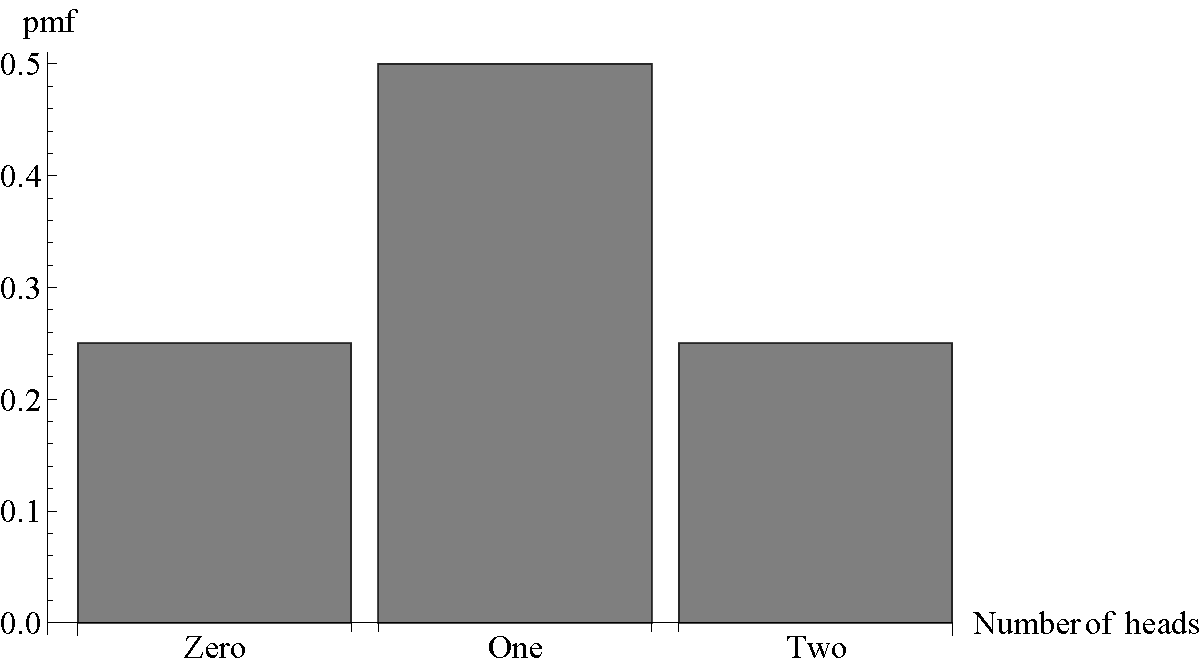
\includegraphics{Likelihood_fairCoin.png}}
\caption{Insert bar chart here of the number of heads along the x axis - 0,1,2 - and the associated probability of each of these outcomes as being the bar height - (1/4,1/2,1/4).}\label{fig:Likelihood_fairCoin}
\end{figure}

\section{Why is a likelihood not a probability for Bayesians?}
When we hold the parameters of our model fixed, as when we held the probability of an individual throw turning up heads to be $\theta=\frac{1}{2}$, we've reasoned that the first term of the numerator of Bayes' rule in (\ref{eq:Likelihood_Bayes}) really is simply a probability. So why don't we just keep calling it that, and forgo the introduction of this new word 'likelihood'? 

The reason is that in Bayesian inference, we \textit{don't} keep the parameters of our model fixed! In Bayesian analysis, it is the \textit{data} that is fixed, and we vary the parameters. Why do we do this? It is because a posterior probability distribution is a probability of a parameter in a model taking on a particular value, across a range of different parameter values. For the case of a coin, where we don't know the probability of a head beforehand, what we hope to get out is a probability distribution of the kind shown in figure \ref{fig:Likelihood_posteriorExample}. Notice that the x-axis in figure \ref{fig:Likelihood_posteriorExample} is the value of $\theta$ - the probability of a heads being obtained. In order to get this posterior probability, $P(\theta|data)$, for each value of theta, we use Bayes' rule in (\ref{eq:Likelihood_Bayes}). This means that for each \textit{different} value of $\theta$, we calculate the first part of the numerator which is $P(data|\theta)$; meaning that we calculate this across a range of $\theta$. If we assume that we have obtained two heads, and vary $\theta$ between 0 and 1 we can obtain the likelihood, which is shown in figure \ref{fig:Likelihood_coinLikelihood}. On first glances in might appear like \ref{fig:Likelihood_coinLikelihood} is a probability distribution, but first looks can be deceiving. 

\begin{figure}
\centering
\scalebox{0.25} 
{\includegraphics{Likelihood_posterior example.png}}
\caption{An example posterior distribution for the probability of a heads.}\label{fig:Likelihood_posteriorExample}
\end{figure}

\begin{figure}
\centering
\scalebox{0.25} 
{\includegraphics{Likelihood_likelihood.png}}
\caption{The x-axis here is theta, ranging between 0 and 1, assuming that one head is obtained this graphs the likelihood, which does not sum to 1.}\label{fig:Likelihood_coinLikelihood}
\end{figure}

Checking off our necessary components of a probability distribution, we first note that all the values of the distribution in figure \ref{fig:Likelihood_coinLikelihood} are non-negative; which is what we require. However, if we look at the area underneath the curve in figure \ref{fig:Likelihood_coinLikelihood}, we find that it does not integrate to 1! Thus we have a violation of the second condition for a valid probability distribution. Hence, when we vary $\theta$ we find that, $P(data|\theta)$ is not a valid probability distribution! We thus introduce the term 'likelihood' to represent value of $P(data|\theta)$ when we vary the parameter, $\theta$. Often the following notation is used to emphasise that likelihood is a function of the parameter $\theta$ with the data held fixed:

\begin{equation}
\mathcal{L}(\theta|data) = P(data|\theta)
\end{equation}\label{eq:Likelihood_notation}

However, in this book, we will persist with the original notation as this is most typical in the literature, under the implicit assumption that when we vary the parameters in question, the term is not strictly a probability.

To provide further justification for this argument, consider the following (albeit contrived) example. Suppose that, we throw a coin twice, and we are told beforehand that the probability of obtaining a head on a particular throw is one of six discrete values: $\theta\in\{0.0,0.2,0.4,0.6,0.8,1.0\}$. In this circumstance, we can calculate the probability of the number of heads, $X$, occurring as:

\begin{align}\label{eq:Likelihood_OneHead}
P(X = 0|\theta)& = P(TT|\theta) = P(T|\theta)\times P(T|\theta) = (1-\theta)^2\\
P(X = 1|\theta)& = P(HT|\theta) + P(TH|\theta) = 2\times P(T|\theta)\times P(H|\theta) = 2\theta(1-\theta)\\\label{eq:Likelihood_TwoHead}
P(X = 2|\theta)& = P(HH|\theta) = P(H|\theta)\times P(H|\theta) = \theta^2
\end{align}

In (\ref{eq:Likelihood_OneHead}), the probability is simply given by the product of the probabilities of not obtaining a head on the first throw, $(1-\theta)$, by the probability of not obtaining a head in the second\footnote{Since we have assumed a model whereby the results of the first and second throws are independent, conditional on $\theta$. In other words, all the similarity between the two throws is captured in the parameter $\theta$.}, which is also $(1-\theta)$. The factor of two arises in (\ref{eq:Likelihood_TwoHead}) since there are two ways of getting one head: \{HT,TH\}.

We can represent the corresponding values of likelihood/probability as in table \ref{tab:Likeihood_BayesBox}. In this form we can see the impact of varying the data (moving along each row), and contrast it with the effect of varying $\theta$ (moving down each column). The important thing to see here is that if we hold the parameter fixed - regardless of this initial choice of $\theta$ - and move along each row summing the entries, we find that the values sum to 1; meaning that this is a proper probability distribution. By contrast, when we hold the number of heads fixed, and vary the parameter $\theta$, moving down each column, summing the entries, we find that the values do not sum to 1. Hence, when we vary $\theta$, we are not dealing with a proper probability distribution, thus meriting the use of the term 'likelihood'.

In Bayesian inference, we always vary the parameter, and implicitly hold the data fixed. Thus, from a Bayesian perspective it is important to use the term Likelihood to indicate that we recognise we are not dealing with a probability distribution.


\begin{table}[htbp]
  \centering
  
    \begin{tabular}{ccccc}
    \multicolumn{5}{c}{\textbf{Number of heads}} \\
    \midrule
    \textbf{$\theta$} & \multicolumn{1}{c}{\textbf{0}} & \multicolumn{1}{c}{\textbf{1}} & \multicolumn{1}{c}{\textbf{2}} &  \multicolumn{1}{c}{\textbf{Total}} \\
    \hline
    \textbf{0.0} & \multicolumn{1}{c}{1.00} & \multicolumn{1}{c}{0.00} & \multicolumn{1}{c}{0.00} & \multicolumn{1}{c}{\textbf{1.00}} \\
    \textbf{0.2} & \multicolumn{1}{c}{0.64} & \multicolumn{1}{c}{0.32} & \multicolumn{1}{c}{0.04} & \multicolumn{1}{c}{\textbf{1.00}} \\
    \textbf{0.4} & \multicolumn{1}{c}{0.36} & \multicolumn{1}{c}{0.48} & \multicolumn{1}{c}{0.16} & \multicolumn{1}{c}{\textbf{1.00}} \\
    \textbf{0.6} & \multicolumn{1}{c}{0.16} & \multicolumn{1}{c}{0.48} & \multicolumn{1}{c}{0.36} & \multicolumn{1}{c}{\textbf{1.00}} \\
    \textbf{0.8} & \multicolumn{1}{c}{0.04} & \multicolumn{1}{c}{0.32} & \multicolumn{1}{c}{0.64} & \multicolumn{1}{c}{\textbf{1.00}} \\
    \textbf{1.0} & \multicolumn{1}{c}{0.00} & \multicolumn{1}{c}{0.00} & \multicolumn{1}{c}{1.00} & \multicolumn{1}{c}{\textbf{1.00}} \\
    \bottomrule
    \textbf{Total} & \multicolumn{1}{c}{\textbf{1.20}} & \multicolumn{1}{c}{\textbf{1.60}} & \multicolumn{1}{c}{\textbf{2.20}} &  \\
    
    \end{tabular}%
  %
  \caption{The values of likelihood for the case of tossing a coin twice, where the probability of heads is constrained to take on a discrete value: \{0.0,0.2,0.4,0.6,0.8,1.0\}. In each of the rows, the value of $theta$ is held constant, meaning that $P(data|\theta)$ is a proper probability distribution and thus the probabilities sum to 1. However, in the columns, the data - the number of heads thrown - is held constant, and thus the probabilities do not sum to 1, and we thus we are better off viewing these data as likelihoods, since they do not satisfy the properties of a proper probability distribution.}\label{tab:Likeihood_BayesBox}
\end{table}

\section{What are models, and why do we need them?}
All models are wrong. They are idealised representations of reality resultant from making assumptions, which if reasonable, may emulate some of the behaviour of a system of interest. Joshua Epstein in an article titled, 'Why model?' emphasises that we perennially build \textit{implicit} mental models for various phenomena \cite{epstein2008model}. Before we go to bed at night we set our alarms for the next morning on the basis of a model. We imagine an idealised - model - morning when it takes us 15 minutes to wake up as a result of an alarm. We use this model to predict how long it will take us to rise from bed, shower, and get changed into clothes in sufficient time to get to work. Whenever we go to the Doctor, they use an internalised biological model of the human body to advise on the best course of treatment for a particular ailment. Whenever we hear expert opinions on TV about the outcome of an upcoming election, the pundits are using mental models of society to explain the results of current polls, as well as make forecasts. As is the case with all models, some of these models are better than others. Hopefully, the models a Doctor uses to prescribe medicine are subject to less error than the opinions of pundits seen on TV! 

Epstein goes on to emphasise that the question, 'Why model?' really means why should we build an \textit{explicit} - written down - model of a phenomena? The point being that \textit{implicit} models are by their very nature, opaque, and not subject to the sort of interrogation and calibration that can be obtained by writing the model on paper. 

We can also ask more narrowly, what are we hoping to gain by building an \textit{explicit} model of a situation? Epstein goes on to suggest 16 reasons, other than prediction, to build a model, of which I list a selected few below:

\begin{itemize}
\item Explain
\item Guide data collection
\item Discover new questions
\item Bound outcomes to plausible ranges
\item Illuminate uncertainties
\item Challenge the robustness of prevailing theory through perturbations
\item Reveal the apparently simple (complex) to be complex (simple) 
\end{itemize}

There are of course other reasons to build models, but I believe that this list encapsulates the majority of them. However, we should not think of this list as static. Whenever we build a model, whether it is statistical, biological or sociological, we should ask, 'What are we hoping to gain by building this model, and how can I judge its success?'. Only when we have a grasp on the answers to these basic questions should we proceed to model building.

\section{How to choose an appropriate model for likelihood?}
Bayesians are acutely aware that their models are wrong. At best, they represent an abstraction from reality, and at worst, they can provide very misleading descriptions of a real phenomenon. Before we use a model for prediction, we should always require that a model is capable of \textit{explanation} of the past and present. With this in mind, I propose the following course of action to specifying a statistical model of which likelihood forms a core part.

\begin{enumerate}
\item Write down the real life behaviour/data patterns that your model should be capable of explaining.
\item Write down the assumptions that we believe are reasonable in order to arrive at such a model.
\item Search for an appropriate/similar model in the literature.
\item Test your model's ability to explain said behaviour/data patterns. If unsuccessful go back to the second step and re-evaluate the appropriateness of your assumptions.
\end{enumerate}

Whilst this methodology is useful for building a statistical model in general, practically how do we go about specifying a likelihood for a given situation? To answer this we will start with going through a simple example.

\subsection{A likelihood model of disease prevalence}
Suppose we work for the NHS and we want to build a simple statistical model which is used to explain the prevalence of a certain disease within a sample, which can then be used to make inferences about the population incidence. Also, (unrealistically) let's assume that we start off by assuming that we have a sample of only one person, of which we have no prior information. Let the disease status of that individual be denoted by the variable $X$ which takes on the following binary outcome values dependent on the disease status the individual:

\begin{equation}
X =
\begin{cases}
O & , No\; disease \\
1 & , Positive \; diagnosis
\end{cases}
\end{equation}

The goal of a likelihood model which we specify is to be able to explain the prevalence of the disease in the population, as well as make predictions about disease incidence in new samples of individuals. We might assume that a fraction $\theta$ of the population has the disease, and that this individual has come from that population. For each possible outcome, we can use this simple model to specify the probability of each outcome:

\begin{align}\label{eq:Likelihood_SimpleModel}
P(X = 0|\theta)& = P(TT|\theta) = P(T|\theta)\times P(T|\theta) = (1-\theta)^2\\
P(X = 1|\theta)& = P(HT|\theta) + P(TH|\theta) = 2\times P(T|\theta)\times P(H|\theta) = 2\theta(1-\theta)\\
P(X = 2|\theta)& = P(HH|\theta) = P(H|\theta)\times P(H|\theta) = \theta^2
\end{align}


\subsection{A likelihood model of wage determinants}


\section{The subjectivity of model choice}
\section{Maximum likelihood - a short introduction}
\section{Chapter summary}


\bibliographystyle{plain}
\bibliography{Bayes}

\end{document}